\documentclass[14pt]{extarticle}
\usepackage{extsizes}
\usepackage[top=0.75in, bottom=0.5in, left=0.5in, right=0.5in]{geometry}
\usepackage{amsmath,amsfonts, color, booktabs, centernot, textcomp,amssymb,graphicx,verbatim,enumerate, bbm}
%\usepackage [autostyle, english = american]{csquotes}
%\usepackage [style = american]{csquotes}
%\MakeOuterQuote{"}
\usepackage{algorithm} % Boxes/formatting around algorithms
\usepackage[noend]{algpseudocode} % Algorithms
\usepackage{wrapfig}
\usepackage{fancyhdr}
\pagestyle{fancy}
\setlength\parindent{0pt}
\setcounter{tocdepth}{3} % should be default
\newcounter{problemnumber}
\def\Name{Leah Dickstein}

\title{Collection of Proofs}
\author{\Name \vspace{-2ex}}
\date{\today}
\lhead{\Name}

\begin{document}
\maketitle

System: \\
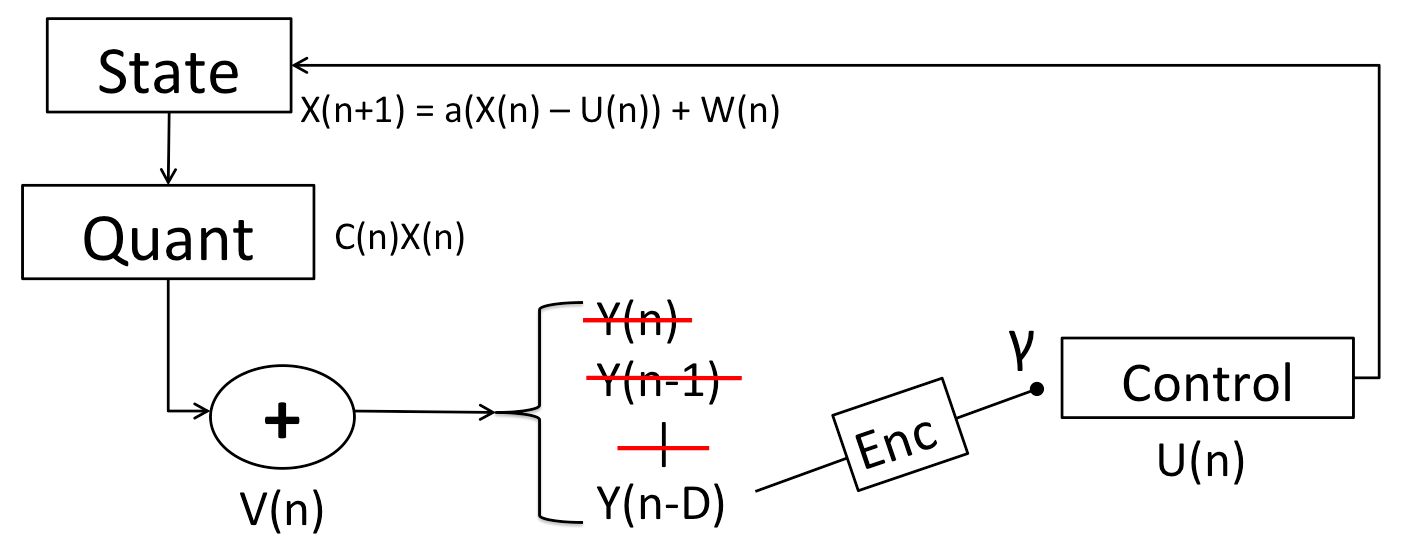
\includegraphics[width=0.5\textwidth]{sys_dynamics}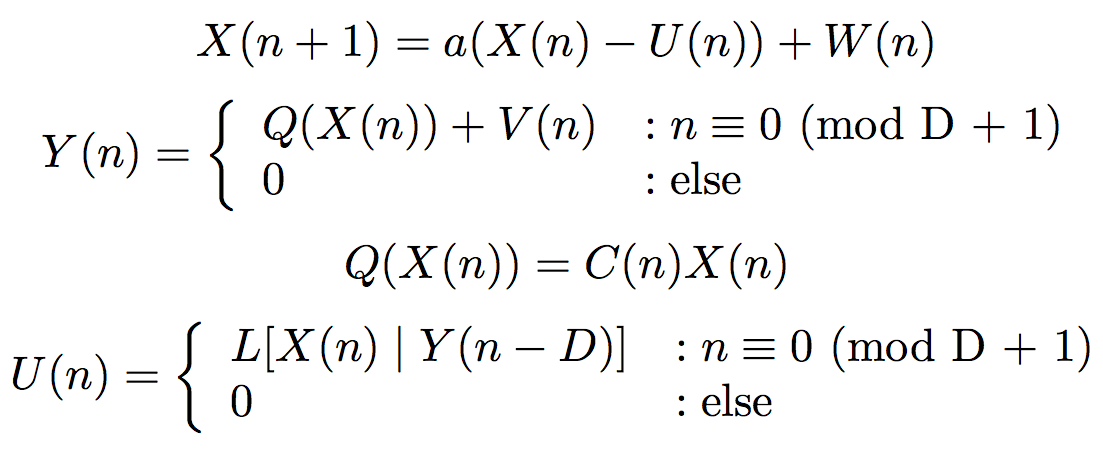
\includegraphics[width=0.5\textwidth]{sys_equations}
% 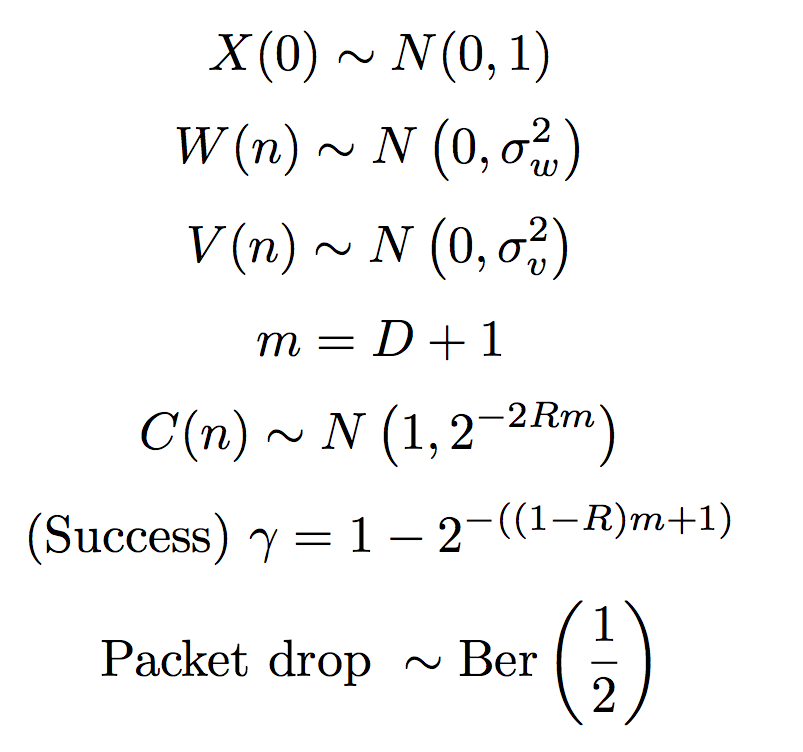
\includegraphics[width=0.35\textwidth]{sys_params}

\tableofcontents

\section*{New Cost Function -- Penalize Large Control Power}

\subsection*{Optimal Control -- No V(n), $\gamma = 1$, No Delay}

\[ \text{min } \mathbb{E} [ x^2(n+1) ] + \sum_{k=1}^n u^2(k) \]

\begin{math}
\text{min } \mathbb{E} [  a( x(n) - u(n) ) + w(n) )^2 ] + \sum_{k=1}^n u^2(k) \\
= \text{min } \mathbb{E} [( a( x(n) - \alpha(n) y(n) ) + w(n) )^2 ] + \sum_{k=1}^n \alpha^2(k) y^2(k) \\
= \text{min } \mathbb{E} [( a( x(n) - \alpha(n) c(n)x(n) ) + w(n) )^2 ] + \sum_{k=1}^n \alpha^2(k) c^2(k) x^2(k) \\
= \text{min } \mathbb{E} [ a^2 (1 - \alpha c(n) )^2 x^2(n) ] + \sigma_w^2 + \sum_{k=1}^n \alpha^2(k) y^2(k) \\
\frac{d}{d \alpha(n)} \mathbb{E} [ a^2 (1 - \alpha(n) c(n) )^2 x^2(n) ] + \sigma_w^2 + \sum_{k=1}^n \alpha^2(k) y^2(k) = \mathbb{E} [2a^2 (1 - \alpha(n) c(n) ) (-c(n)) x^2(n) ] + 2 \alpha(n) y^2(n)= 0 \\
-a^2 ( \mu_c \sigma_{x(n)}^2 - \alpha(n) (\mu_c^2 + \sigma_c^2 ) \sigma_{x(n)}^2 ) + \alpha(n) y^2(n) = 0 \\
\alpha(n) (a^2 (\mu_c^2 + \sigma_c^2 ) \sigma_{x(n)}^2 + y^2(n) ) = a^2 \mu_c \sigma_{x(n)}^2
\end{math}

\[ \alpha(n) = \frac{a^2 \mu_c \sigma_{x(n)}^2}{a^2 (\mu_c^2 + \sigma_c^2) \sigma_{x(n)}^2 + y^2(n)} \]

This is easy to implement, and my next step is to implement this. My worry is that this isn't a closed solution like the previous $\alpha$ calculations. As time passes, $\alpha$ will change every time a new control is implemented--which is fine, but we should note the new complication. Does this answer make sense? Should I go ahead and implement this?

\subsection*{A Bound -- No V(n), $\gamma = 1$, No Delay}

\[ \alpha(n) = \frac{a^2 \mu_c \sigma_{x(n)}^2}{a^2 (\mu_c^2 + \sigma_c^2) \sigma_{x(n)}^2 + y^2(n)} \]

\begin{math}
\mathbb{E} [x^2(n+1)] \\
= \mathbb{E} [( ax(n) - a\alpha y(n) + w(n) )^2] \\
= \mathbb{E} [( ax(n) - a\alpha c(n)x(n) + w(n) )^2] \\
= \mathbb{E} [( a(1-\alpha c(n))x(n) + w(n) )^2 ] \\
a^2 (1 - 2\alpha \mu_c + \alpha^2 (\mu_c^2 + \sigma_c^2) ) < 1
\end{math}

\[ a^2 \left( 1 - \frac{2 a^2 \mu_c^2 \sigma_{x(n)}^2}{a^2 (\mu_c^2 + \sigma_c^2) \sigma_{x(n)}^2 + y^2(n)} + \frac{a^4 \mu_c^2 \sigma_{x(n)}^4 (\mu_c^2 + \sigma_c^2) }{(a^2 (\mu_c^2 + \sigma_c^2) \sigma_{x(n)}^2 + y^2(n))^2} \right) < 1 \]

As this is similar to original cost function with V(n), I don't believe this is easily simplifiable. This should just be calculated in code/implementation.

\section*{Original Cost Function: Minimize Mean Square State}

\subsection*{Optimal Control -- No V(n), $\gamma = 1$, Delay}

\[ \text{min } \mathbb{E} [x^2(n+1) ] \]

\begin{math}
\text{min } \mathbb{E} [( a (x(n) - \alpha y(n-D) ) + w(n) )^2 ] \\
= \text{min } \mathbb{E} [( a (x(n) - \alpha c(n-D)x(n-D) ) + w(n) )^2] \\
= \text{min } \mathbb{E} [( a (a^Dx(n-D) + \sum_{i=1}^D a^{i-1} w(n-i) - \alpha c(n-D)x(n-D) ) + w(n) )^2] \\
= \text{min } \mathbb{E} [( a(a^D - \alpha c(n-D) x(n-D) + \sum_{i=0}^D a^i w(n-i) )^2 ] \\
\frac{d}{d \alpha} \downarrow = \mathbb{E} [2a^2 (a^D - \alpha c(n-D) ) x^2(n-D) (-c(n-D)) ] = 0 \\
\mathbb{E}[c(n-D) (a^D - \alpha c(n-D)) x^2(n-D) ] = 0 \\
a^D \mu_c \sigma^2_{x(n-D)} = \alpha (\mu_c^2 + \sigma_c^2) \sigma^2_{x(n-D)}
\end{math}

\[ \alpha = \frac{a^D \mu_c}{\mu_c^2 + \sigma_c^2} \]

The addition of delay simply means our control has to project into the future (by a scaling factor) for when it will be applied.

\subsection*{A Bound -- No V(n), $\gamma = 1$, Delay}

\[ \alpha = \frac{a^D \mu_c}{\mu_c^2 + \sigma_c^2} \]

\begin{math}
\mathbb{E} [( a(x(n) - \alpha y(n-D)) + w(n) )^2] \\
= \mathbb{E} [( ax(n) - a\alpha y(n-D) + w(n) )^2] \\
= \mathbb{E} [( a^{D+1}x(n-D) - a\alpha y(n-D) + \sum_{i=0}^D a^i w(n-i) )^2 ] \\
= \mathbb{E} [( a^{D+1}x(n-D) -a\alpha c(n-D)x(n-D) + \sum_{i=0}^D a^i w(n-i) )^2] \\
= \mathbb{E} [(a^{D+1} - a\alpha c(n-D))^2 x^2(n-D) ] + \mathbb{E} [\sum_{i=0}^D a^{2i} w^2(n-i) ] \\
a^{2(D+1)} - 2a^{D+2} \alpha \mu_c + a^2 \alpha^2 (\mu_c^2 + \sigma_c^2 ) < 1 \\
a^{2(D+1)} - \frac{2a^{2(D+1)} \mu_c^2}{\mu_c^2 + \sigma_c^2} + \frac{a^{2(D+1)} \mu_c^2}{\mu_c^2 + \sigma_c^2} < 1 \\
a^{2(D+1)} - \frac{a^{2(D+1)} \mu_c^2}{\mu_c^2 + \sigma_c^2} < 1 \; \rightarrow \;  a^{2(D+1)} \left( 1 - \frac{\mu_c^2}{\mu_c^2 + \sigma_c^2} \right) < 1 \; \rightarrow \; a^{2(D+1)} < \frac{\mu_c^2 + \sigma_c^2}{\sigma_c^2}
\end{math}

\[  a^{2(D+1)} < \frac{\mu_c^2 + \sigma_c^2}{\sigma_c^2} \quad \quad a < \left( \frac{\mu_c^2 + \sigma_c^2}{\sigma_c^2} \right)^{\frac{1}{2(D+1)}} \]

\subsection*{Optimal Control -- No V(n), $\gamma = 1$, No Delay}

\[ \text{min } \mathbb{E} [x^2(n+1) ] \]
\[ u(n) = \alpha y(n) = \alpha c(n) x(n) \]

\begin{math}
\text{min } \mathbb{E} [( a( x(n) - u(n) ) + w(n) )^2 ] \\
= \text{min } \mathbb{E} [( a( x(n) - \alpha y(n) ) + w(n) )^2 ] \\
= \text{min } \mathbb{E} [( a( x(n) - \alpha c(n)x(n) ) + w(n) )^2 ] \\
= \text{min } \mathbb{E} [ a^2 (1 - \alpha c(n) )^2 x^2(n) ] + \sigma_w^2 \\
\frac{d}{d \alpha} \mathbb{E} [ a^2 (1 - \alpha c(n) )^2 x^2(n) ] + \sigma_w^2 = \mathbb{E} [2a^2 (1 - \alpha c(n) ) (-c(n)) x^2(n) ] = 0 \\
\mathbb{E} [c(n) x^2(n) - \alpha c^2(n) x^2(n) ] = 0 \\
\mu_c \sigma_{x(n)}^2 = \alpha (\mu_c^2 + \sigma_c^2 ) \sigma_{x(n)}^2
\end{math}

\[ \alpha = \frac{\mu_c}{\mu_c^2 + \sigma_c^2} \]

These are the results we expect, from Gireeja's Noncoherence Paper.

\subsection*{Optimal Control -- V(n), $\gamma = 1$, Delay}

\[ \text{min } \mathbb{E} [x^2(n+1) ] \]

\begin{math}
\text{min } \mathbb{E} [( ax(n) - a\alpha y(n-D) + w(n) )^2] \\
= \text{min } \mathbb{E} [( a^{D+1}x(n-D) + \sum_{i=0}^D a^i w(n-i) -a\alpha y(n-D) )^2 ] \\
= \text{min } \mathbb{E} [( a^{D+1}x(n-D) -a\alpha c(n-D)x(n-D) -a\alpha v(n-D) + \sum_{i=0}^D a^i w(n-i) )^2] \\
\frac{d}{d\alpha} \downarrow = \mathbb{E} [-2a^{D+2} c(n-D) x^2(n-D) + 2\alpha a^2 c^2(n-D) x^2(n-D) + 2a^2 \alpha v^2(n-D) ] = 0 \\
-a^{D+2} \mu_c \sigma_{x(n-D)}^2 + \alpha a^2 (\mu_c^2 + \sigma_c^2) \sigma^2_{x(n-D)} + \alpha a^2 \sigma_v^2 = 0 \\
\alpha ( (\mu_c^2 + \sigma_c^2) \sigma_{x(n-D)}^2 + \sigma_v^2 ) = a^D \mu_c \sigma^2_{x(n-D)}
\end{math}

\[ \alpha(n) = \frac{a^D \mu_c \sigma_{x(n-D)}^2}{(\mu_c^2 + \sigma_c^2) \sigma_{x(n-D)}^2 + \sigma_v^2} \]

\subsection*{A Bound -- V(n), $\gamma = 1$, Delay}

\[ \alpha(n) = \frac{a^D \mu_c \sigma_{x(n-D)}^2}{(\mu_c^2 + \sigma_c^2) \sigma_{x(n-D)}^2 + \sigma_v^2} \]

\begin{math}
\mathbb{E} [a^{2(D+1)}x^2(n-D) -2a^{D+2}\alpha(n) c(n-D) x^2(n-D) + a^2 \alpha^2(n) c^2(n-D) x^2(n-D) ] \\
a^{2(D+1)} - 2a^{D+2} \alpha(n) \mu_c + a^2 \alpha^2(n) (\mu_c^2 + \sigma_c^2) < 1 \\
a^{2(D+1)} - \frac{2a^{2(D+1)} \mu_c \sigma^2_{x(n-D)}}{(\mu_c^2 + \sigma_c^2) \sigma_{x(n-D)}^2 + \sigma_v^2 } + \frac{a^{2(D+1)} \mu_c^2 \sigma^4_{x(n-D)} (\mu_c^2 + \sigma_c^2)}{((\mu_c^2 + \sigma_c^2) \sigma_{x(n-D)}^2 + \sigma_v^2)^2} < 1
\end{math}

\[ a^{2(D+1)} \left( 1 - \frac{2\mu_c^2 \sigma^2_{x(n-D)}}{(\mu_c^2+\sigma_c^2) \sigma^2_{x(n-D)} + \sigma_v^2} + \frac{\mu_c^2 \sigma^4_{x(n-D)} (\mu_c^2 + \sigma_c^2)}{((\mu_c^2 + \sigma_c^2) \sigma^2_{x(n-D)} + \sigma_v^2 )^2} \right) < 1 \]

This is really ugly. I started looking into simplifying it, but I don't think it can be simplified further. It would be best to directly calculate everything out in implementation/code. 

\subsection*{Optimal Control -- V(n) $\gamma = 1$, No Delay}

\[ \text{min } \mathbb{E} [x^2(n+1) ] \]

\begin{math}
\text{min } \mathbb{E} [ ( a(1-\alpha c(n) ) x(n) - a\alpha v(n) + w(n) )^2 ] \\
= \text{min } \mathbb{E}[ a^2 (1-\alpha c(n) )^2 x^2(n) + \mathbb{E} [a^2 \alpha^2 v^2(n) ] + \sigma_w^2 \\
\frac{d}{d \alpha}  \mathbb{E}[ a^2 (1-\alpha c(n) )^2 x^2(n) + \mathbb{E} [a^2 \alpha^2 v^2(n) ] + \sigma_w^2 = \mathbb{E}[ -2a^2 (1-\alpha c(n)) c(n) x^2(n) ] + 2 a^2 \alpha \sigma_v^2 = 0\\
= -\mu_c \sigma_{x(n)}^2 + \alpha (\mu_c^2 + \sigma_c^2 ) \sigma_{x(n)}^2 + \alpha \sigma_v^2 = 0
\end{math}

\[ \alpha(n) = \frac{\mu_c \sigma_{x(n)}^2}{(\mu_c^2 + \sigma_c^2) \sigma_{x(n)}^2 + \sigma_v^2} \]

These are the results we expect from the LLSE theorem: $\alpha = \frac{cov(X, Y)}{var(Y)} = \frac{\mathbb{E}[XY]}{\mathbb{E}[Y^2]} \leftarrow \text{assuming } \mathbb{E}[X] = \mathbb{E}[Y] = 0 $

\end{document}